\section{Технический проект}

\subsection{Общие сведения о программно-информационной системе}

Полное наименование системы: Веб-приложение "Социомаркет для владельцев домашних животных".

Краткое обозначение системы: "Социомаркет".

Описание системы: "Социомаркет" предназначена для владельцев домашних животных, предоставляя им платформу для поиска и предложения различных услуг и товаров для животных. Система создана для облегчения доступа к широкому спектру услуг, от ветеринарной помощи до груминга и других товаров для животных.

Условия эксплуатации: "Социомаркет" предназначена для использования в нормальных условиях работы, доступна через веб-браузеры на персональных компьютерах и мобильных устройствах.

Архитектура системы: Программное обеспечение основано на клиент-серверной архитектуре, используя современные технологии веб-разработки, включая .NET Core для серверной части и Angular для клиентской части. Система поддерживает REST API для обеспечения взаимодействия между клиентом и сервером и использует базу данных PostgreSQL.

Технологии и инструменты: В разработке использовались Angular, HTML, JavaScript, SCSS для клиентской части, а также .NET Core и Entity Framework Core для серверной части. Для управления данными использовалась технология ORM (Object-Relational Mapping).

Особенности системы:
\begin{itemize}
    \item возможность авторизации для пользователей и поставщиков услуг;
    \item разработка удобного интерфейса для поиска продуктов (товаров и услуг);
    \item возможность управления карточками услуг и товаров для поставщиков;
\end{itemize}

\subsection{Обоснование выбора технологий проектирования}
\subsubsection{.NET Core}
Выбор .NET Core для серверной разработки обосновывается его производительностью, масштабируемостью и кросс-платформенностью, а также поддержкой работы с админ-панелью <<из коробки>>, что является важным фактором в современной разработке программного обеспечения \cite{mark_price}.
Начиная с версии .NET core 6.0, которая была выбрана для разработки, поддерживается работа с админ-панелью <<из коробки>>, что позволяет сэкономить ресурсы на разработки панели администратора.

\subsubsection{Entity Framework Core}
Entity Framework Core является ORM (Object-Relational Mapping) для .NET Core. Он позволяет работать с базами данных, используя объектно-ориентированный подход \cite{grinchenko}. Entity Framework Core позволяет работать с различными СУБД, в том числе с PostgreSQL, которая была выбрана для разработки. EF Core предоставляет удобные и мощные инструменты для разработки приложений, использующих CRUD подход.

\subsubsection{PostgreSQL}
Выбор PostgreSQL в качестве системы управления базами данных был обусловлен её высокой надежностью, поддержкой продвинутых SQL-функций и совместимостью с EF Core. PostgreSQL предлагает удобные функции для разработчиков, такие как JSON/JSONB поддержка, хранение процедур и триггеры, что делает её идеальной для комплексных приложений, требующих масштабируемости и гибкости. К тому же, PostgreSQL обладает мощными средствами для работы с большими объемами данных и комплексными запросами, что критично для обеспечения высокой производительности приложения.

\subsubsection{Angular}
Angular, выбранный для Frontend разработки, предоставляет строгую и требовательную архитектуру, что делает его идеальным инструментом для создания сложных и масштабируемых приложений. Эффективность Angular в разработке интерактивных интерфейсов и легкость интеграции с REST API подчеркивается. Angular предоставляет возможность писать код на TypeScript, что упрощает разработку и поддержку приложения и обеспечивает более строгую реализацию принципов ООП в клиенской части приложения.

\subsection{Проектирование пользовательского интерфейса}

На основании требований к пользовательскому интерфейсу, представленных в пункте 2.3 технического задания, был разработан графический интерфейс мобильного приложения, используя Angular с применением HTML, JavaScript и SCSS \cite{cssspecs}. Этот процесс подчеркивает важность интуитивно понятного и эффективного взаимодействия с пользователем \cite{kumskova}.
Разработанный интерфейс ориентирован на обеспечение легкости в использовании и интуитивного понимания функционала приложения, предоставляя пользователю гладкое и эффективное взаимодействие с приложением.

\begin{enumerate}
    \item \textbf{Поиск}: Реализация функции поиска на основе поля \textit{ProductName} из класса \textit{Product}, \textit{Price}, \textit{Weight}, и \textit{ProductGroupId} класса \textit{Product};
    \item \textbf{Отображение результатов поиска}: Эффективное представление списка товаров, включая \textit{ImageUrl}, \textit{ProductName}, информацию о \textit{Category} и \textit{Price};
    \item \textbf{Детали товара}: Дополнительная информация о товаре, включая его \textit{Category} и \textit{Weight};
    \item \textbf{Навигация по приложению}: Элементы навигации, такие как кнопка возврата к началу списка и индикаторы категорий.
\end{enumerate}

\begin{figure}[h!]
    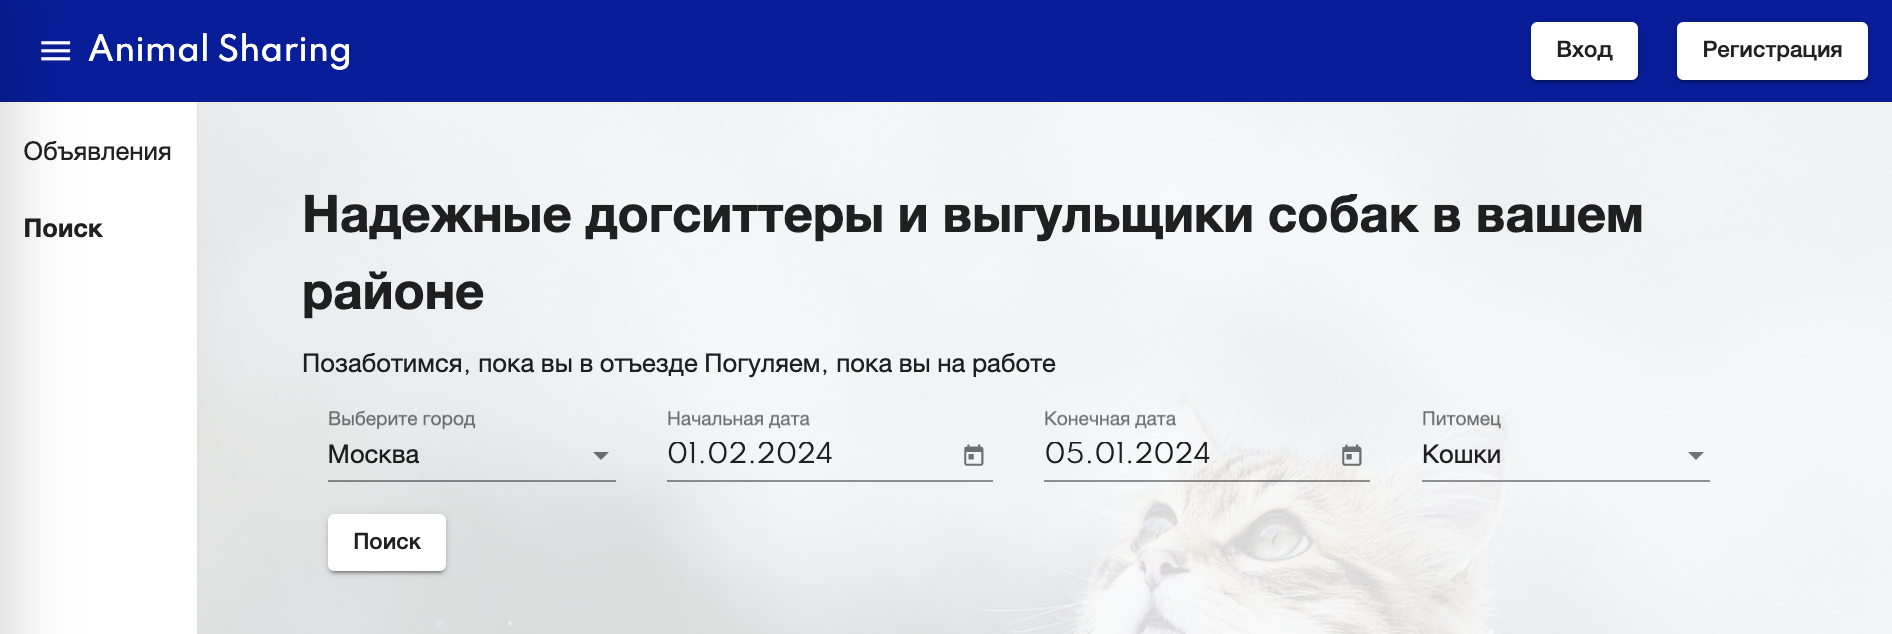
\includegraphics[width=0.82\linewidth]{interface-search.jpg}
    \caption{модели интерфейса <<Поиск>> и <<Навигация по приложению>>}
    \label{fig:search}
\end{figure}

Процесс регистрации пользователя в приложении максимально упрощен и включает следующие шаги:
\begin{enumerate}
    \item Пользователь выбирает опцию <<Регистрация>> на главном экране;
    \item Заполняются основные поля: электронная почта, имя пользователя и пароль;
    \item Пользователь должен подтвердить свой адрес электронной почты через полученное письмо со ссылкой для подтверждения;
    \item После подтверждения электронной почты, пользователь может ввести дополнительную информацию в свой профиль: фотографию, контактные данные и предпочтения в приложении;
    \item На последнем этапе пользователь принимает условия пользования и политику конфиденциальности, после чего регистрация завершается.
\end{enumerate}

Регистрация дог-ситтеров предполагает прохождение дополнительных этапов для верификации и предоставления информации о предоставляемых услугах:
\begin{enumerate}
    \item Потенциальный дог-ситтер начинает регистрацию с выбора соответствующего пункта в приложении;
    \item Вводятся личные данные, включая полное имя, адрес проживания и номер телефона;
    \item Запрашивается информация о предыдущем опыте работы с животными и наличии соответствующих рекомендаций;
    \item Дог-ситтер должен пройти онлайн-курс по уходу за животными и предоставить сертификат о его окончании;
    \item Предоставляется информация об услугах, включая доступные даты и временные рамки, а также устанавливаются тарифы;
    \item Профиль дог-ситтера отправляется на проверку. После одобрения администрацией профиль становится доступным для поиска и выбора пользователями.
\end{enumerate}


\begin{figure}[h!]
    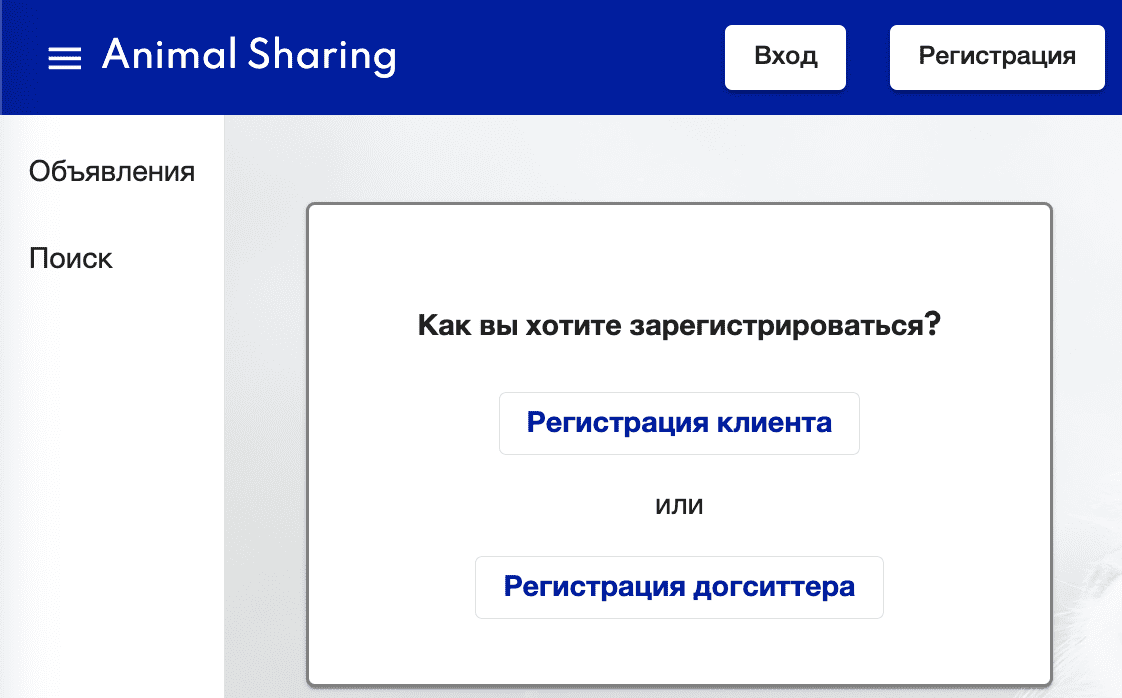
\includegraphics[width=0.82\linewidth]{interface-register}
    \caption{Модели интерфейса регистрации <<Пользователя>> и <<Дог-ситтера>>}
    \label{fig:register}
\end{figure}

\subsection{Диаграмма размещения}

Диаграмма размещения, отображаемая на рисунке \ref{place:image}, является фундаментальным инструментом для иллюстрации взаимосвязей между программными и аппаратными компонентами системы. Этот элемент визуализации служит для акцентирования значимости стратегического планирования в процессе разработки распределенных систем. Детальное и глубокое понимание этих взаимосвязей критически важно для успешного создания и функционирования распределенных информационных систем\cite{makni}. Каждый компонент системы, будь то программный или аппаратный, играет важную роль в обеспечении её общей эффективности и надежности. Подход, основанный на стратегическом планировании, способствует оптимизации этих взаимодействий и повышает вероятность успешной реализации и эксплуатации системы в целом.

\begin{figure}[ht]
\center{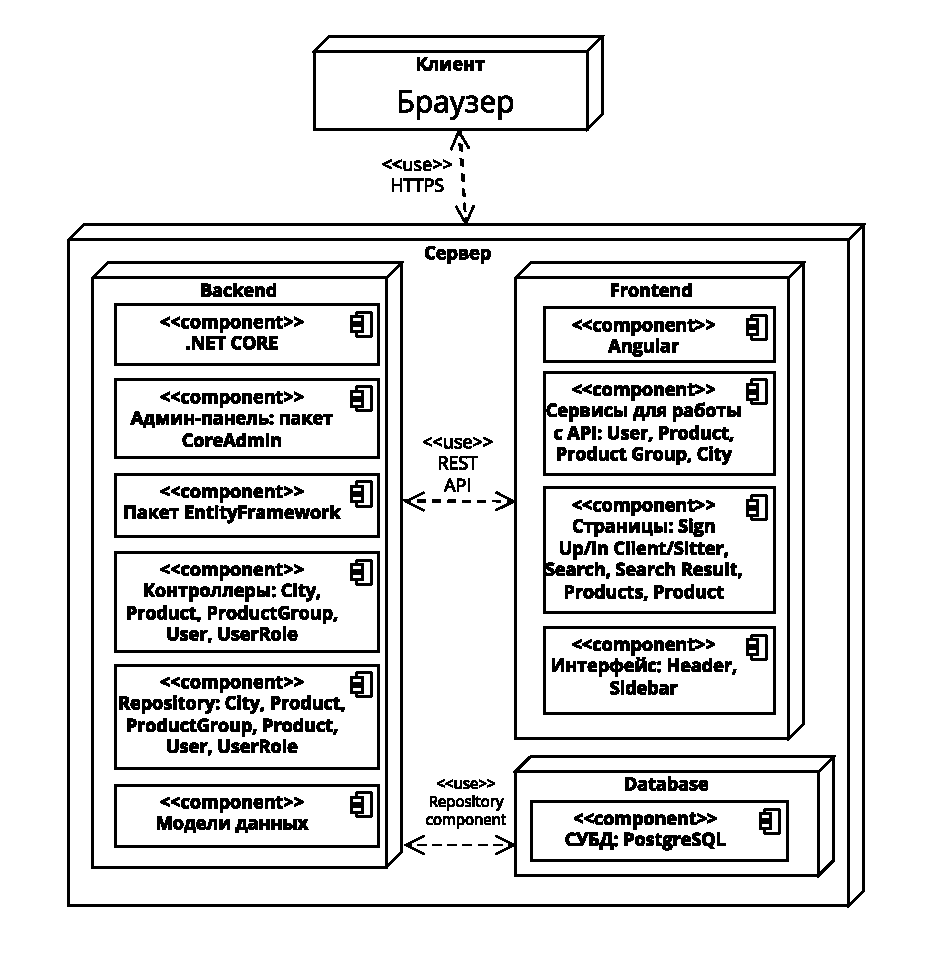
\includegraphics[width=1\linewidth]{client-server.eps}}
\caption{Диаграмма размещения}
\label{place:image}
\end{figure}

Она является хорошим средством для показа маршрутов перемещения объектов и компонентов в распределенной системе.

\subsection{Описание классов системы}

\subsubsection{Описание программных классов серверной части}

\begin{itemize}
    \item <<UserBase>> является фундаментальным классом для хранения пользовательских данных. Помимо основных свойств, таких как <<Phone>>, <<Email>>, <<FirstName>>, <<LastName>>, предлагает основу для дальнейшего расширения и интеграции с другими подсистемами приложения.
    \item <<UserRegistrationData>> расширяет <<UserBase>>, вводя специфические свойства, необходимые для процесса регистрации, включая <<Password>>. Это обеспечивает дополнительный уровень безопасности и индивидуализации данных пользователя.
    \item <<UserLoginData>> применяется для авторизации пользователей в системе. Содержит только самую необходимую информацию для входа, а именно: <<Email>> и <<Password>>.
    \item <<UserLoginResponseData>> и <<UserView>> наследуются от <<UserBase>> и дополняют его уникальным идентификатором <<Id>>. <<UserLoginResponseData>> также включает в себя <<AccessToken>>, что обеспечивает надежную аутентификацию и безопасность данных.
    \item <<User>> представляет собой полную структуру класса пользователя, включая элементы безопасности (<<Hash>> и <<Salt>>) и уникальный идентификатор <<Id>>. Этот класс является центральным в системе управления пользователями и их данными.
\end{itemize}

% Таблица для HashSalt
\begin{xltabular}{\textwidth}{|l|l|p{1.7cm}|X|}
    \caption{Свойства класса <<HashSalt>>}\label{hashsalt:table} \\ \hline
    Свойство & Тип & \makecell{Обяза-\\тельное} & Описание \\ \hline
    1 & 2 & 3 & 4 \\ \hline
    \finishhead
    Hash & String & true & Хэш \\ \hline
    Salt & String & true & Соль для хэша \\ \hline
\end{xltabular}

% Таблица для UserBase
\begin{xltabular}{\textwidth}{|l|l|p{1.7cm}|X|}
    \caption{Свойства класса <<UserBase>>}\label{userbase:table} \\ \hline
    Свойство & Тип & \makecell{Обяза-\\тельное} & Описание \\ \hline
    1 & 2 & 3 & 4 \\ \hline
    \endfirsthead
    1 & 2 & 3 & 4 \\ \hline
    \finishhead
    Phone & String & false & Телефонный номер пользователя \\ \hline
    Email & String & false & Электронная почта пользователя \\ \hline
    FirstName & String & false & Имя пользователя \\ \hline
    LastName & String & false & Фамилия пользователя \\ \hline
    ImageUrl & String & false & URL изображения пользователя \\ \hline
    Telegram & String & false & Telegram пользователя \\ \hline
    Website & String & false & Веб-сайт пользователя \\ \hline
\end{xltabular}

% Таблица для UserRegistrationData
\begin{xltabular}{\textwidth}{|l|l|p{1.7cm}|X|}
    \caption{Свойства класса <<UserRegistrationData>>}\label{userregdata:table} \\ \hline
    Свойство & Тип & \makecell{Обяза-\\тельное} & Описание \\ \hline
    1 & 2 & 3 & 4 \\ \hline
    Password & String & true & Пароль пользователя \\ \hline
\end{xltabular}

% Таблица для UserLoginData
\begin{xltabular}{\textwidth}{|l|l|p{1.7cm}|X|}
    \caption{Свойства класса <<UserLoginData>>}\label{userlogindata:table} \\ \hline
    Свойство & Тип & \makecell{Обяза-\\тельное} & Описание \\ \hline
    1 & 2 & 3 & 4 \\ \hline
    Email & String & true & Электронная почта пользователя для входа \\ \hline
    Password & String & true & Пароль пользователя для входа \\ \hline
\end{xltabular}

% Таблица для UserLoginResponseData
\begin{xltabular}{\textwidth}{|l|l|p{1.7cm}|X|}
    \caption{Свойства класса <<UserLoginResponseData>>}\label{userloginrespdata:table} \\ \hline
    Свойство & Тип & \makecell{Обяза-\\тельное} & Описание \\ \hline
    1 & 2 & 3 & 4 \\ \hline
    Id & Long & true & Уникальный идентификатор пользователя \\ \hline
    AccessToken & String & true & Токен доступа пользователя \\ \hline
\end{xltabular}

% Таблица для UserView
\begin{xltabular}{\textwidth}{|l|l|p{1.7cm}|X|}
    \caption{Свойства класса <<UserView>>}\label{userview:table} \\ \hline
    Свойство & Тип & \makecell{Обяза-\\тельное} & Описание \\ \hline
    1 & 2 & 3 & 4 \\ \hline
    Id & Long & true & Уникальный идентификатор пользователя \\ \hline
\end{xltabular}

% Таблица для User
\begin{xltabular}{\textwidth}{|l|l|p{1.7cm}|X|}
    \caption{Свойства класса <<User>>}\label{user:table} \\ \hline
    Свойство & Тип & \makecell{Обяза-\\тельное} & Описание \\ \hline
    1 & 2 & 3 & 4 \\ \hline
    \endfirsthead
    1 & 2 & 3 & 4 \\ \hline
    \finishhead
    Id & Long & true & Уникальный идентификатор пользователя \\ \hline
    Hash & String & true & Хэш пользователя \\ \hline
    Salt & String & true & Соль для хэша пароля пользователя \\ \hline
\end{xltabular}

Большой набор классов для описания пользователя в серверной части приложение таких как <<UserBase>>, <<UserRegistrationData>>, <<UserLoginData>>, <<UserLoginResponseData>> и <<User>>, подчеркивает разнообразие и сложность структур данных в современных системах. Подход к проектированию \cite{grinchenko} и реализации этих классов основывается на объектно-ориентированных принципах и практиках \cite{kumskova}.

В частности, класс <<User>> является центральным в системе управления пользователями и их данными, что подчеркивает важность его реализации и интеграции с другими классами.

% Таблица для Product
\begin{xltabular}{\textwidth}{|l|l|p{1.7cm}|X|}
    \caption{Свойства класса <<Product>>}\label{product:table} \\ \hline
    Свойство & Тип & \makecell{Обяза-\\тельное} & Описание \\ \hline
    1 & 2 & 3 & 4 \\ \hline
    \endfirsthead
    1 & 2 & 3 & 4 \\ \hline
    \finishhead
    ImageUrl & String & false & URL изображения продукта \\ \hline
    ProductGroupId & Long & true & Идентификатор группы продуктов \\ \hline
    Price & Float & true & Цена продукта \\ \hline
    Weight & Integer & true & Вес продукта \\ \hline
    CreatedByUserId & Long & true & Идентификатор пользователя, создавшего продукт \\ \hline
\end{xltabular}

% Таблица для ProductView
\begin{xltabular}{\textwidth}{|l|l|p{1.7cm}|X|}
    \caption{Свойства класса <<ProductView>>}\label{productview:table} \\ \hline
    Свойство & Тип & \makecell{Обяза-\\тельное} & Описание \\ \hline
    1 & 2 & 3 & 4 \\ \hline
    CreatedByUser & UserView & true & Пользователь, создавший продукт \\ \hline
\end{xltabular}

\begin{itemize}
    \item <<Product>>, наследующийся от <<Short>>, описывает основные свойства продукта, такие как <<ImageUrl>>, <<ProductGroupId>>, <<Price>>, <<Weight>>, и <<CreatedByUserId>>, указывающий на пользователя, создавшего продукт.
    \item <<ProductView>> расширяет <<Product>>, добавляя <<CreatedByUser>>, который является экземпляром <<UserView>>. Это позволяет получать не только идентификационную информацию о создателе продукта, но и более детальные данные пользователя.
\end{itemize}

% Таблица для IUserRepository
\begin{xltabular}{\textwidth}{|l|l|p{1.7cm}|X|}
    \caption{Свойства класса <<IUserRepository>>}\label{iuserrepository:table} \\ \hline
    Свойство & Тип & \makecell{Обяза-\\тельное} & Описание \\ \hline
    1 & 2 & 3 & 4 \\ \hline
    \endfirsthead
    1 & 2 & 3 & 4 \\ \hline
    \finishhead
    GetById & User & true & Получить пользователя по идентификатору \\ \hline
    GetByEmail & User & true & Получить пользователя по электронной почте \\ \hline
    GetAllUserViews & List<UserView> & true & Получить список пользователей \\ \hline
    Create & User & true & Создать пользователя \\ \hline
\end{xltabular}

Класс <<IUserRepository>> описывает основные методы для работы с пользователями, включая получение пользователя по идентификатору, получение пользователя по электронной почте, получение списка пользователей и создание пользователя.

В системе предусмотрен внутренний механизм связи между классами и их свойствами, поэтому введение дополнительных идентификаторов при реализации связей между классами не предполагается.

Экземпляры классов реализуются в информационных блоках посредством элементов, свойства класса – посредством свойств и методов элемента.

\subsubsection{Описание программных классов клиентской части}

\begin{itemize}
    \item <<Short>> - основной класс, используемый для предоставления общей структуры данных. Свойства <<id>>, <<name>> и <<description>> являются фундаментальными для большинства классов;
    \item <<User>> - расширяет <<Short>>, интегрируя контактные данные и личную информацию пользователя. Используется для управления учетными записями пользователей, включая процессы регистрации и авторизации;
    \item <<ProductGroup>> - расширяет <<Short>>, добавляя конкретные детали для организации продуктов в группы. Используется для классификации и управления ассортиментом продуктов;
    \item <<Product>> - расширяет <<Short>>, предоставляя подробную информацию о продуктах. Включает данные о создателе продукта и используется для представления конкретных товаров в системе;
    \item <<City>> - описывает города, со свойствами <<id>> и <<name>>. Используется для управления информацией о местоположениях, связанных с пользователями и продуктами.
    \item <<ProductFilter>> - используется для фильтрации продуктов по городу, группе продуктов, дате публикации и дате окончания срока действия.
\end{itemize}

% Таблица для Short
\begin{xltabular}{\textwidth}{|l|l|p{1.7cm}|X|}
    \caption{Свойства класса <<Short>>\label{int1:table}}\\ \hline
    Свойство & Тип & \makecell{Обяза-\\тельное} & Описание \\ \hline
    1 & 2 & 3 & 4 \\ \hline
    \endfirsthead
    1 & 2 & 3 & 4 \\ \hline
    \finishhead
    id & number & true & Уникальный идентификатор \\ \hline
    name & string & true & Название \\ \hline
    description & string & true & Описание \\ \hline
\end{xltabular}

% Таблица для User
\begin{xltabular}{\textwidth}{|l|l|p{1.7cm}|X|}
    \caption{Свойства класса <<User>>\label{int2:table}}\\ \hline
    Свойство & Тип & \makecell{Обяза-\\тельное} & Описание \\ \hline
    1 & 2 & 3 & 4 \\ \hline
    \endfirsthead
    1 & 2 & 3 & 4 \\ \hline
    \finishhead
    phone & string & true & Телефонный номер \\ \hline
    email & string & true & Электронная почта \\ \hline
    firstName & string & true & Имя \\ \hline
    lastName & string & true & Фамилия \\ \hline
    photoUrl & string & true & URL изображения \\ \hline
    telegram & string & true & Telegram \\ \hline
    website & string & true & Веб-сайт \\ \hline
    address & string & true & Адрес \\ \hline
    userRoleId & number & true & Идентификатор роли \\ \hline
    password & string & false & Пароль пользователя (передается при авторизации и регистрации) \\ \hline
    accessToken & string & false & Токен доступа (принимается при авторизации и регистрации) \\ \hline
\end{xltabular}

% Таблица для Product
\begin{xltabular}{\textwidth}{|l|l|p{1.7cm}|X|}
    \caption{Свойства класса <<Product>>\label{int3:table}}\\ \hline
    Свойство & Тип & \makecell{Обяза-\\тельное} & Описание \\ \hline
    1 & 2 & 3 & 4 \\ \hline
    \endfirsthead
    1 & 2 & 3 & 4 \\ \hline
    \finishhead
    imageUrl & string & true & URL изображения продукта \\ \hline
    productGroupId & number & true & Идентификатор группы продуктов \\ \hline
    price & number & true & Цена продукта \\ \hline
    weight & number & true & Вес продукта \\ \hline
    createdByUserId & number & true & Идентификатор пользователя, создавшего продукт \\ \hline
    publishedAt & Date & true & Дата публикации \\ \hline
    expiredAt & Date & true & Дата окончания срока действия \\ \hline
\end{xltabular}

% Таблица для ProductGroup
\begin{xltabular}{\textwidth}{|l|l|p{1.7cm}|X|}
    \caption{Свойства класса <<ProductGroup>>\label{int4:table}}\\ \hline
    Свойство & Тип & \makecell{Обяза-\\тельное} & Описание \\ \hline
    1 & 2 & 3 & 4 \\ \hline
    \endfirsthead
    1 & 2 & 3 & 4 \\ \hline
    \finishhead
    type & string & true & Тип группы продуктов \\ \hline
    childrenProductGroupIds & number[] & true & Идентификаторы дочерних групп продуктов (может быть пустым массивом) \\ \hline
    parentProductGroupId & number & false & Идентификатор родительской группы продуктов \\ \hline
\end{xltabular}

% Таблица для ProductFilter
\begin{xltabular}{\textwidth}{|l|l|p{1.7cm}|X|}
    \caption{Свойства класса <<ProductFilter>>\label{int5:table}}\\ \hline
    Свойство & Тип & \makecell{Обяза-\\тельное} & Описание \\ \hline
    1 & 2 & 3 & 4 \\ \hline
    \endfirsthead
    1 & 2 & 3 & 4 \\ \hline
    \finishhead
    cityId & number & false & Идентификатор города \\ \hline
    productGroupId & number & false & Идентификатор группы продуктов \\ \hline
    publishedAtFrom & Date & false & Дата публикации \\ \hline
    expiredAtTo & Date & false & Дата окончания срока действия \\ \hline
\end{xltabular}

% Таблица для City
\begin{xltabular}{\textwidth}{|l|l|p{1.7cm}|X|}
    \caption{Свойства класса <<City>>\label{int6:table}}\\ \hline
    Свойство & Тип & \makecell{Обяза-\\тельное} & Описание \\ \hline
    1 & 2 & 3 & 4 \\ \hline
    id & number & true & Уникальный идентификатор \\ \hline
    name & string & true & Название города \\ \hline
\end{xltabular}

% Таблица для UserService
\begin{xltabular}{\textwidth}{|l|l|p{1.7cm}|X|}
    \caption{Свойства класса <<UserService>>\label{int6:table}}\\ \hline
    Свойство & Тип & \makecell{Обяза-\\тельное} & Описание \\ \hline
    1 & 2 & 3 & 4 \\ \hline
    \endfirsthead
    1 & 2 & 3 & 4 \\ \hline
    \finishhead
    getById & User & true & Получить пользователя по идентификатору \\ \hline
    login & User & true & Получить пользователя по электронной почте \\ \hline
    create & User & true & Получить список пользователей \\ \hline
    update & User & true & Создать пользователя \\ \hline
\end{xltabular}

% Таблица для ProductGroupService
\begin{xltabular}{\textwidth}{|l|l|p{1.7cm}|X|}
    \caption{Свойства класса <<ProductGroupService>>\label{int7:table}}\\ \hline
    Метод & Тип & \makecell{Обяза-\\тельное} & Описание \\ \hline
    1 & 2 & 3 & 4 \\ \hline
    \endfirsthead
    1 & 2 & 3 & 4 \\ \hline
    \finishhead
    getAll & ProductGroup[] & true & Получить все группы продуктов \\ \hline
    updateAll & ProductGroup[] & true & Обновить все группы продуктов \\ \hline
\end{xltabular}

% Таблица для ProductService
\begin{xltabular}{\textwidth}{|l|l|p{1.7cm}|X|}
    \caption{Свойства класса <<ProductService>>\label{int8:table}}\\ \hline
    Метод & Тип & \makecell{Обяза-\\тельное} & Описание \\ \hline
    1 & 2 & 3 & 4 \\ \hline
    \endfirsthead
    1 & 2 & 3 & 4 \\ \hline
    \finishhead
    getAll & Product[] & true & Получить все продукты \\ \hline
    getById & Product & true & Получить продукт по идентификатору \\ \hline
    add & Product & true & Добавить продукт \\ \hline
    update & Product & true & Обновить продукт \\ \hline
    delete & void & true & Удалить продукт \\ \hline
    getFilteredProducts & Product[] & true & Получить отфильтрованные продукты \\ \hline
\end{xltabular}

% Таблица для CityService
\begin{xltabular}{\textwidth}{|l|l|p{1.7cm}|X|}
    \caption{Свойства класса <<CityService>>\label{int9:table}}\\ \hline
    Метод & Тип & \makecell{Обяза-\\тельное} & Описание \\ \hline
    1 & 2 & 3 & 4 \\ \hline
    getAll & City[] & true & Получить все города \\ \hline
\end{xltabular}

Классы <<UserService>>, <<ProductGroupService>>, <<ProductService>> и <<CityService>> предоставляют методы для отправки HTTP запросов к API серверной части приложения.